\documentclass[11pt]{beamer}
\usepackage[T1]{fontenc}
\usepackage{hyperref}
\usepackage{url}
\usepackage{xcolor}
\usepackage[linesnumbered, ruled, longend]{algorithm2e}
\usepackage{colortbl}
\usepackage{subcaption}
\usepackage{amsmath,amssymb}
\usepackage{ragged2e}
\usepackage{etoolbox}
\usepackage{multirow}
\renewcommand{\raggedright}{\leftskip=0pt \rightskip=0pt plus 0cm}
\apptocmd{\frame}{}{\justifying}{}
\let\oldenumerate=\enumerate 
\renewenvironment{enumerate}{\oldenumerate\raggedright}{\endlist} 
\let\olditemize=\itemize
\renewenvironment{itemize}{\olditemize\raggedright}{\endlist}

\usepackage{xcolor}
\definecolor{commentgreen}{RGB}{2,112,10}
\definecolor{eminence}{RGB}{108,48,130}
\definecolor{weborange}{RGB}{255,165,0}
\definecolor{frenchplum}{RGB}{129,20,83}

\usepackage{listings}
\usepackage{textcomp}
\lstset {
	language=Java,
	frame=tb,
	tabsize=4,
	showstringspaces=false,
	numbers=left,
	upquote=true,
	commentstyle=\color{commentgreen},
	keywordstyle=\color{eminence},
	stringstyle=\color{red},
	basicstyle=\small\ttfamily, % basic font setting
	emph={int,char,double,float,unsigned,void,bool},
	emphstyle={\color{blue}},
	escapechar=\&,
	% keyword highlighting
	classoffset=1, % starting new class
	morekeywords={>,<,.,;,,,-,!,=,~},
	keywordstyle=\color{weborange},
	classoffset=0,
}

\usepackage{adjustbox}
\newcommand{\code}[1]{\texttt{#1}}

\usetheme{Warsaw}
\useoutertheme{smoothtree}
\usepackage[utf8]{vietnam}
%%%%%%%%%%%%%%%%%%%%%%%%%%%%%%%%%%%%
\def\mydate{\leavevmode\hbox{\bfseries\the\day/\twodigits\month/\twodigits\year}}
\def\twodigits#1{\ifnum#1<10 0\fi\the#1}
%%%%%%%%%%%%%%%%%%%%%%%%%%%%%%%%%%%%
\definecolor{sectioncolor}{RGB}{39,0,118}
\definecolor{framecolor}{RGB}{37,109,255}

\setbeamercolor{frametitle}{fg=white, bg=blue}
\definecolor{light-gray}{gray}{0.95}
%%%%%%%%%%%%%%%%%%%%%%%%%%%%%%%%%%%
\setbeamertemplate{footline}
{%
	\leavevmode%
	\begin{beamercolorbox}[wd=.5\paperwidth,ht=2.75ex,dp=1.5ex]{author in head/foot}%
		\hbox to .5\paperwidth{\hfil\insertshortauthor\hfil}
	\end{beamercolorbox}%
	\begin{beamercolorbox}[wd=.5\paperwidth,ht=2.75ex,dp=1.5ex]{date in head/foot}%
		\raggedleft
		\usebeamerfont{date in head/foot}
		\insertframenumber{} / \inserttotalframenumber\hspace*{15pt}
	\end{beamercolorbox}%
}
\begin{document}
\author[Nhóm 13]{
	Giảng viên hướng dẫn: TS. Nguyễn Thị Thu Trang
	\vspace{.5in} 
	\begin{columns}
		\begin{column}{.5\linewidth}
			\centering
			Nhóm sinh viên
		\end{column}
		\begin{column}{.55\linewidth}
			1. Phạm Minh Khiêm - 20170084\\
			2. Lê Vũ Lợi - 20173240\\
			3. Phạm Trung Kiên - 20170088
		\end{column}
	\end{columns}
}
\title[]{\bfseries\fontsize{14}{\baselineskip}\selectfont BÁO CÁO BÀI TẬP LỚN\vspace{5pt}}
\subtitle{Môn học: Thiết kế xây dựng phần mềm}
\logo{
\includegraphics[scale=.1]{Images/SoICTlogo.jpg}}
\institute[\bfseries Viện CNTT\&TT]{}
\date[\mydate]{\today}
%\subject{Yo!}

\begin{frame}[plain]
	\maketitle
\end{frame}
%%%%%%%%%%%%%%%%%%%%%%%%%%%%%%%%%%%%%
\begin{frame}[plain]
	\frametitle{Phân công công việc}
	\begin{itemize}
		\item Lợi: đặc tả usecase Xem chi tiết xe đang thuê, code frontend, thiết kế chi tiết lớp, làm slide. (35\%)
		\item Khiêm: đặc tả usecase Trả xe, code backend, thiết kế giao diện người dùng. (40\%)
		\item Kiên: đặc tả usecase Thuê xe, thiết kế dữ liệu.(25\%)
	\end{itemize}
\end{frame}
%%%%%%%%%%%%%%%%%%%%%%%%%%%%%%%%%%%%%
\begin{frame}[plain]
	\frametitle{Hệ thống cho thuê xe đạp theo giờ}
	\framesubtitle{Biểu đồ usecase tổng quan}
%	\hspace*{-.5in}
	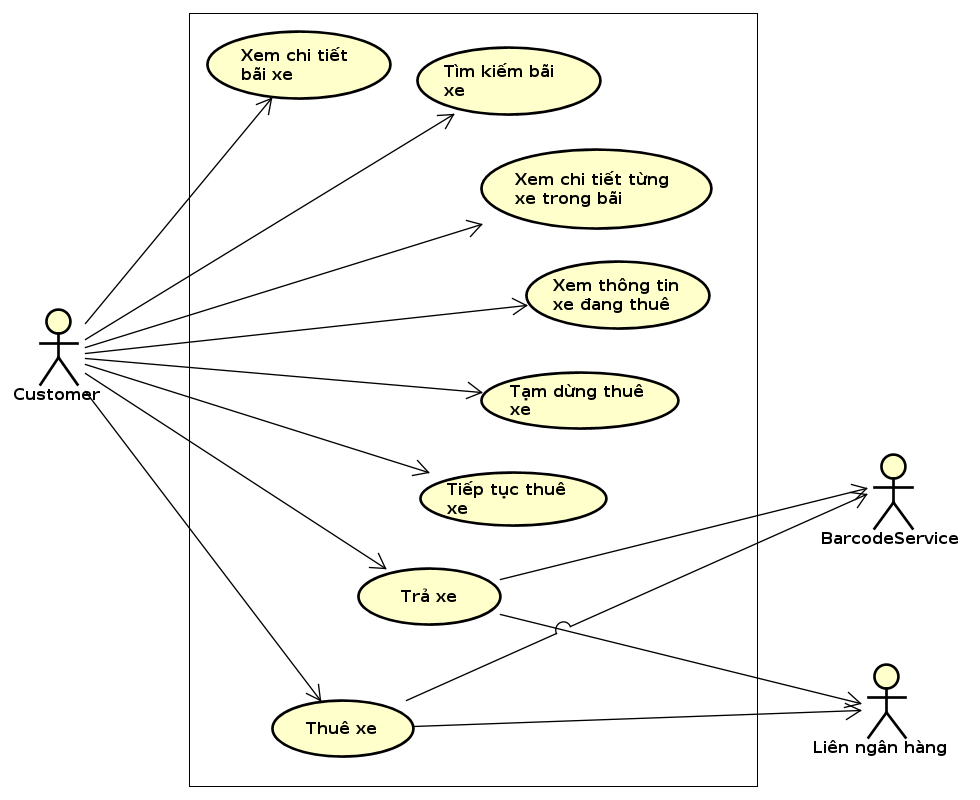
\includegraphics[scale=.35]{Images/Overview.png}
\end{frame}
%%%%%%%%%%%%%%%%%%%%%%%%%%%%%%%%%%%%%
\begin{frame}[plain]
	\frametitle{Phân tích usecase thuê xe}
	\framesubtitle{Biểu đồ trình tự}
	\hspace*{-.1 in}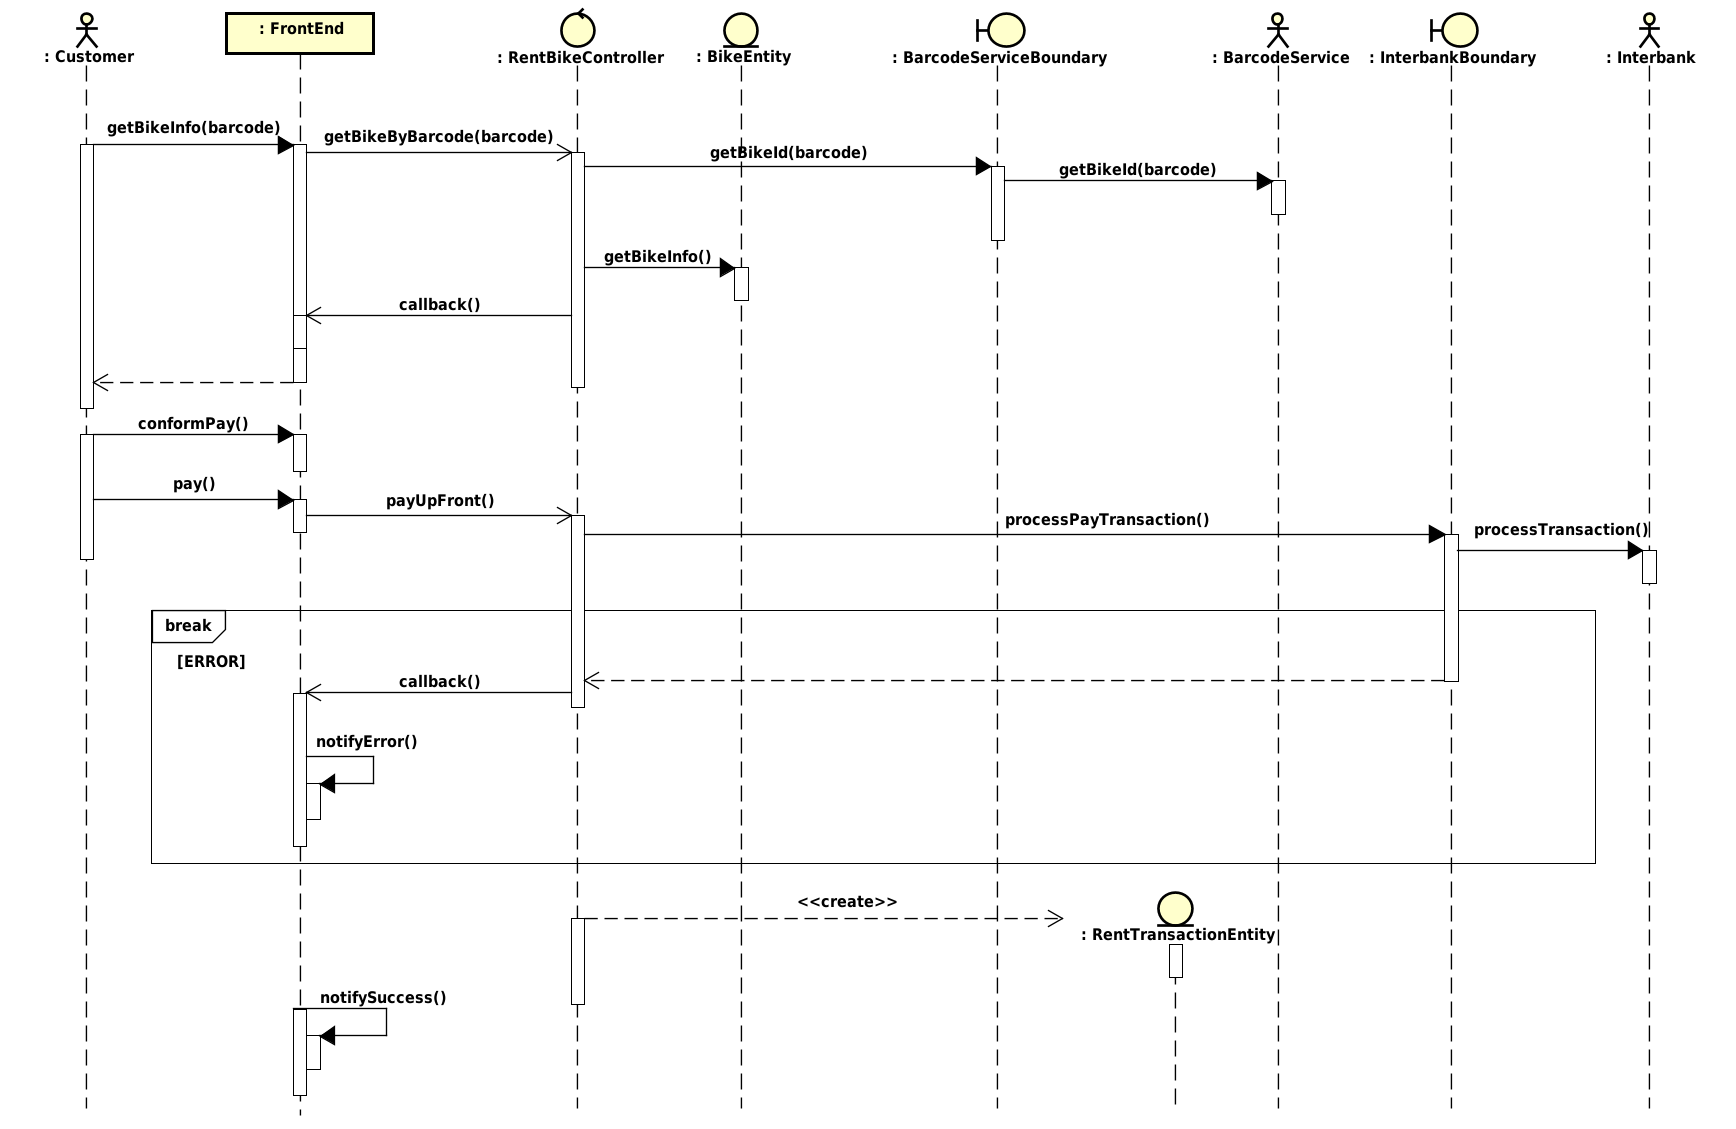
\includegraphics[scale=.25]{Images/RentBike.png}
\end{frame}
%%%%%%%%%%%%%%%%%%%%%%%%%%%%%%%%%%%%%
\begin{frame}[plain]
	\frametitle{Phân tích usecase thuê xe}
	\framesubtitle{Biểu đồ lớp}
	\hspace*{-.1 in}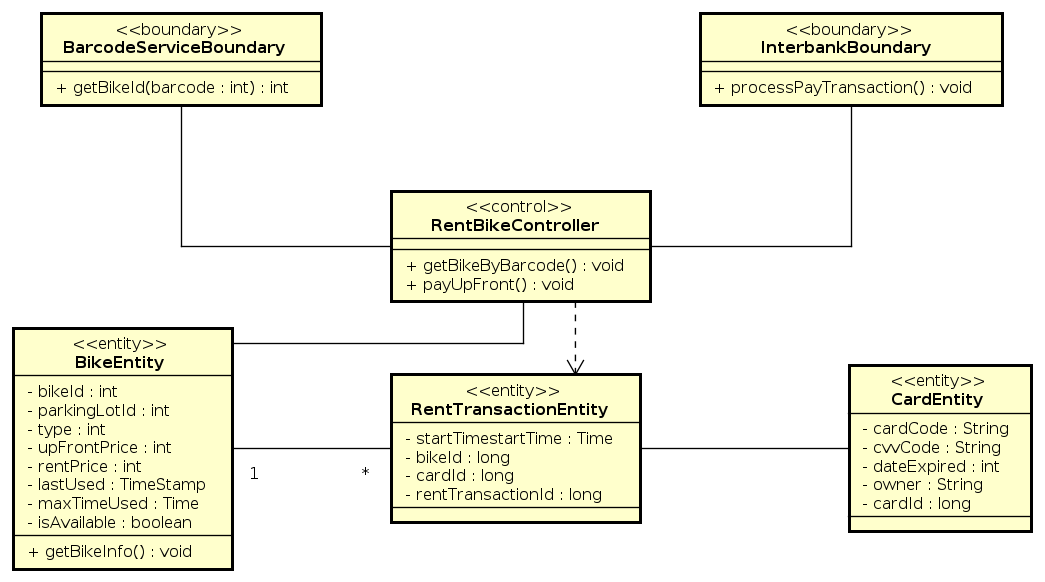
\includegraphics[scale=.4]{Images/RentBikeClass.png}
\end{frame}
%%%%%%%%%%%%%%%%%%%%%%%%%%%%%%%%%%%%%
\begin{frame}[plain]
	\frametitle{Các vấn đề thiết kế}
	\framesubtitle{Design concepts (cohesion and coupling)}
	\begin{itemize}
		\item \textbf{Cohesion}: Các phương thức và thuộc tính của một lớp nếu chỉ được gọi đến ngay bên trong lớp thì sẽ được đặt là private. Điều này làm tăng cohesion bên trong mỗi lớp, đồng thời cũng giảm coupling giữa các lớp với nhau. Ví dụ:\\[10pt]
		\begin{itemize}
			\item Lớp \textit{InterbankController} có phương thức \textit{processTransaction} được để là private. Phương thức này được gọi bởi 2 phương thức public khác là \textit{processPayTransaction} và \textit{processReturnTransaction}.\\[5pt]
			\item Lớp \textit{PaymentController} có các phương thức \textit{payUpFront} và \textit{finalPay} được để là private, lần lượt sử dụng bởi 2 phương thức public khác là \textit{payUpFrontControl} và \textit{finalPayControl}.\\[5pt]
			\item Trong lớp \textit{HttpConnector}, thuộc tính \textit{client} được để private và chỉ phục vụ mục đích sử dụng bên trong lớp này.
		\end{itemize}
	\end{itemize}
\end{frame}
%%%%%%%%%%%%%%%%%%%%%%%%%%%%%%%%%%%%%
\begin{frame}[plain]
	\frametitle{Các vấn đề thiết kế}
	\framesubtitle{Design concepts (cohesion and coupling)}
	\begin{itemize}
		\item \textbf{Coupling}: Mỗi lớp trong hệ thống đều chỉ cung cấp các API public ra bên ngoài, các dữ liệu và logic được ẩn đi ở bên trong. Điều này làm giảm sự phụ thuộc giữa các lớp với nhau, ví dụ:\\[10pt]
		\begin{itemize}
			\item Trong lớp \textit{PaymentController}, nếu cần thay đổi phương thức \textit{payUpFront}, chỉ cần có một thay đổi nhỏ kéo theo trong phương thức \textit{payUpFrontControl} mà không làm ảnh hưởng đến bất kỳ thành phần nào khác của hệ thống.\\[5pt]
			\item Giữa lớp \textit{PaymentController} và \textit{InterbankSystemController}, sự phụ thuộc là gián tiếp thông qua interface \textit{InterbankInterface}. Như vậy, khi thay có thay đổi bên \textit{InterbankSystemController}, các thay đổi này sẽ không làm ảnh hưởng đến \textit{PaymentController}.
		\end{itemize}
	\end{itemize}
\end{frame}
%%%%%%%%%%%%%%%%%%%%%%%%%%%%%%%%%%%%%
\begin{frame}[plain]
	\frametitle{Các vấn đề thiết kế}
	\framesubtitle{Design principles - SOLID}
	\begin{itemize}
		\item \textbf{Single responsibility}\\[10pt]
		\begin{itemize}
			\item Trách nhiệm của hệ thống được phân chia cho từng package và cho từng lớp trong package, cụ thể:\\[8pt]
			\begin{itemize}
				\item Package \textit{controller}: làm nhiệm vụ thực thi các logic của toàn bộ hệ thống.
				\item Package \textit{utils}: chứa các chức năng tiện ích có thể được dùng bởi nhiêu lớp của nhiều gói khác nhau.
				\item Package \textit{entity}: chứa các đối tượng mapping với các bảng trong cơ sở dữ liệu.
				\item Package \textit{repository}: chứa các interface điều khiển việc truy vấn cơ sở dữ liệu. 
				\item Package \textit{Interbank subsystem}: chứa các lớp phục vụ cho việc giao tiếp giữa hệ thống với backend server.
			\end{itemize}
		\end{itemize}
	\end{itemize}
\end{frame}
%%%%%%%%%%%%%%%%%%%%%%%%%%%%%%%%%%%%%
\begin{frame}[plain]
	\frametitle{Các vấn đề thiết kế}
	\framesubtitle{Design principles - SOLID}
	\begin{itemize}
		\item \textbf{Open/closed principle}
		\begin{itemize}
			\item Nguyên tắc này được thực hiện thông qua việc sử dụng các interface.
			\item \textit{Interbank subsystem implement} các phương thức định nghĩa trong \textit{Interbank interface}. Các lớp của hệ thống chỉ phụ thuộc vào Interbank interface chứ không phụ thuộc trực tiếp vào \textit{Interbank subsystem}. Do đó, các sửa chữa và mở rộng sau này đối với \textit{Interbank subsystem} có thể được thực hiện dễ dàng.
		\end{itemize}
	\end{itemize}
\end{frame}
%%%%%%%%%%%%%%%%%%%%%%%%%%%%%%%%%%%%%
\begin{frame}[plain]
	\frametitle{Các vấn đề thiết kế}
	\framesubtitle{Design principles - SOLID}
	\begin{itemize}
		\item \textbf{Liskov substitution principle}
		\begin{itemize}
			\item Nguyên tắc này yêu cầu một lớp con kế thừa từ một lớp cha sẽ có thể sử dụng để thay thế
lớp cha trong bất kì tình huống nào.\\[5pt]
			\item Để đảm bảo yêu cầu này thì đối với các phương thức ghi đè, tham số truyền vào cho lớp con phải có miền giá trị rộng hơn lớp cha, đồng thời giá trị trả về trong phương thức ở lớp con phải có miền giá trị nhỏ hơn.\\[5pt]
			\item Trong thiết kế của hệ thống, lớp \textit{PaymentController} có một thuộc tính tên \textit{interbankSubsystem} với kiểu dữ liệu là \textit{InterbankInterface}. Trong mọi tình huống, kiểu dữ liệu của \textit{interbankSubsystem} có thể chuyển thành \textit{InterbankController}  hay bất kì lớp nào khác implement \textit{InterbankInterface}.
		\end{itemize}
	\end{itemize}
\end{frame}
%%%%%%%%%%%%%%%%%%%%%%%%%%%%%%%%%%%%%
\begin{frame}[plain]
	\frametitle{Các vấn đề thiết kế}
	\framesubtitle{Design principles - SOLID}
	\begin{itemize}
		\item \textbf{Interface segregation principle}
		\begin{itemize}
			\item Một interface không nên chứa quá nhiều phương thức, nếu không các implementations của interface đó có thể bị trùng lặp mã nguồn.\\[5pt]
			\item Trong thiết kế của hệ thống, \textit{InterbankInterface} có 3 phương thức. Các implementations khác của interface nhiều khả năng sẽ khác nhau ở cả 3 phương thức. Do vậy, việc phân chia interface của \textit{InterbankInterface} là hợp lý theo nguyên tắc \textit{Interface segregation}\\[5pt]
		\end{itemize}
	\end{itemize}
\end{frame}
%%%%%%%%%%%%%%%%%%%%%%%%%%%%%%%%%%%%%
\begin{frame}[plain]
	\frametitle{Các vấn đề thiết kế}
	\framesubtitle{Design principles - SOLID}
	\begin{itemize}
		\item \textbf{Dependency inversion principle}
		\begin{itemize}
			\item Các lớp ở tầng trên không nên sử dụng trực tiếp dịch vụ cung cấp bởi các lớp tầng dưới mà nên thông qua một interface.\\[5pt]
			\item Trong thiết kế hiện tại, các lớp sử dụng Java persistence API (trong gói \textit{repository}) sẽ không cần phải thay đổi nếu hệ thống chuyển từ MySQL sang SQLServer. Các lớp sử dụng gói repository như \textit{PaymentController, BikeController} khi cần kết nối đến cơ sở dữ liệu sẽ thông qua đối tượng của gói \textit{repository}.\\[5pt]
		\end{itemize}
	\end{itemize}
\end{frame}
%%%%%%%%%%%%%%%%%%%%%%%%%%%%%%%%%%%%%
\begin{frame}[plain]
	\frametitle{Các vấn đề thiết kế}
	\framesubtitle{Design patterns}
	\begin{itemize}
		\item \textbf{Thư viện \textit{Simple Logging Facade for Java - SLF4J}}
		\begin{itemize}
			\item \textit{Singleton design pattern}: {\tt LoggerFactory.getLogger(Class<> clazz)} - trả về một logger tương ứng với tên lớp được truyền vào. \\[5pt]
			\item \textit{Facade design pattern}: Toàn bộ logic phức tạp của thư viên được đóng gói và cung cấp một API cho người dùng để có thể dễ dàng sử dụng. \\[5pt]
			\item \textit{Factory method}: SLF4J sử dụng \textit{LoggerFactory} để tạo các logger. Người dùng có thể hoàn toàn không quan tâm đến đến các logger được tạo ra mà chỉ cần biết cách để sử dụng chúng. 
		\end{itemize}
	\end{itemize}
\end{frame}
%%%%%%%%%%%%%%%%%%%%%%%%%%%%%%%%%%%%%
\begin{frame}[plain]
	\frametitle{Các vấn đề thiết kế}
	\framesubtitle{Design patterns}
	\begin{itemize}
		\item \textbf{Thư viện \textit{Java Persistence API - JPA}}
		\begin{itemize}
			\item \textit{Singleton design pattern}: Các đối tượng \textit{repository} được gắn với annotation \textbf{@Autowired}. Nếu có 2 lớp cùng sử dụng đối tượng của một lớp \textit{repository}, đối tượng repository này sẽ chỉ được tạo ra một lần cho cả 2 lớp. 
		\end{itemize}
	\end{itemize}
\end{frame}
\end{document}